\chapter{DT workflow in bioprocessing domains} \label{apd:workflow}
The 5D model introduced in Section \ref{sec:overview} provides a reference for entity management in DTs. Nonetheless, in the field of bioprcessing, there are other aspects at which one often finds important to inspect. One of them is the maturity of the DT models. For this reason, Udugama et al. \cite{Udugama2021} propose a five-step workflow (illustrated in Figure \ref{fig:fivestep}) to implement a DT of bioprocessing domain. The workflow progresses in increasing order of mathematical complexity and functional requirements.

\begin{figure}[hbt!]
  \centering
  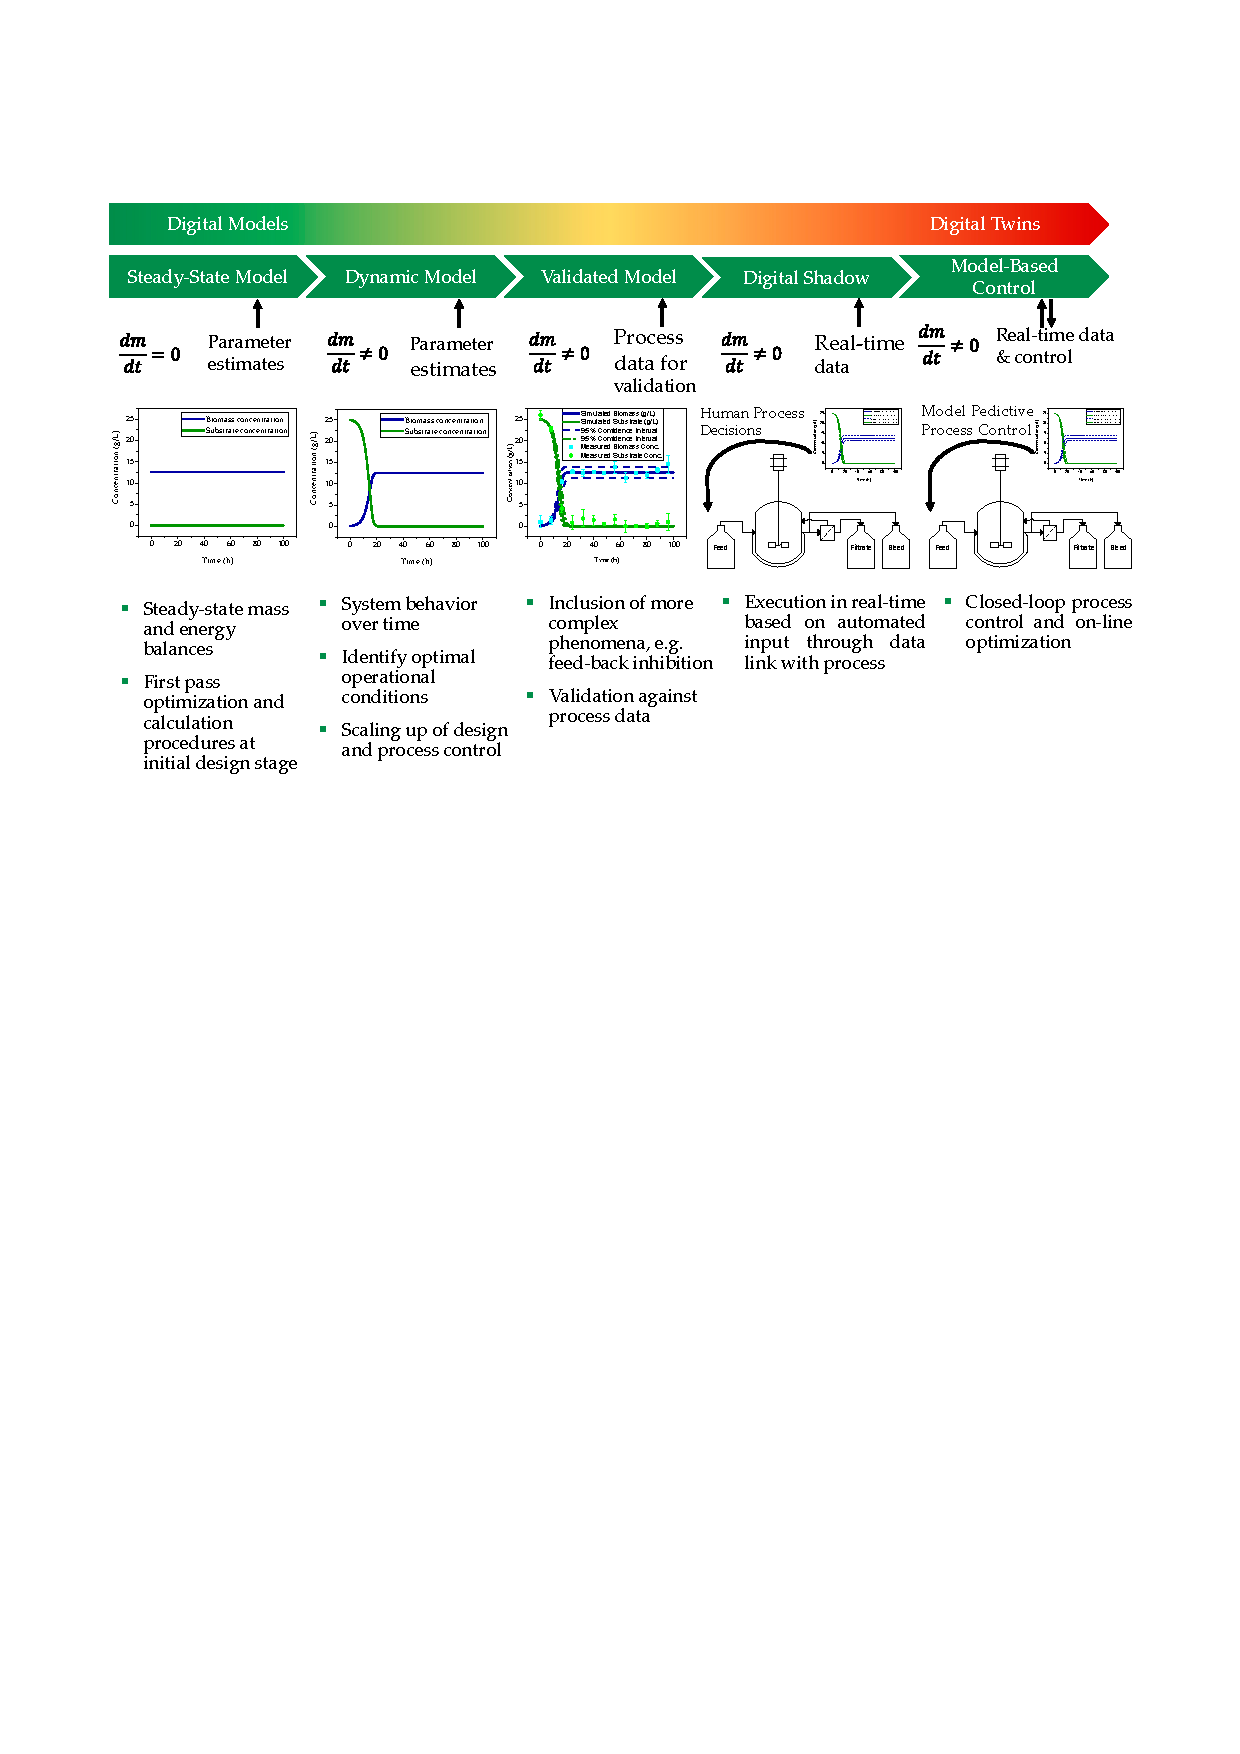
\includegraphics[scale=0.8]{figures/fivestep.pdf}
  \caption[The five-step implementation]{The five-step implementation. This workflow has been adopted in a design of DT for monoclonal antibodies manufacturing \cite{Helgers2022}.}
  \label{fig:fivestep}
\end{figure}

\begin{enumerate}
  \item \textbf{Steady‑state model}: consisted of a mass and energy balance of the different key compounds in a reaction. These models are mathematical expressions of a process
that are not time-dependent and hence carry no accumulation
term.
  \item \textbf{Dynamic model}: contains time-based derivative terms on all variables of interest.
  \item \textbf{Validated model}: extends the capabilities of dynamic process models, such that it needs to be validated against process data obtained from an actual physical process.
  \item \textbf{Digital Shadow}: consistent with the definition of Section \ref{sec:overview}; An one-way real-time monitoring model.
  \item \textbf{Digital Twin}: consistent with the definition of Section \ref{sec:overview}; A two-way real-time monitoring and control model.
\end{enumerate}

\chapter{Microbrewery physical workbench} \label{apd:workbench}
This section presents the workbench setup of the microbrewery DT. All the equipment are settled in a typical living room. A Raspberry Pi is used for aggregating all sensor data (except for those come from Airlock, they use a dedicated webhook server which is included as a part of product supports) before further processing in the DT. Figure \ref{fig:workbench_fermenter} shows the fermenter setup. 

\begin{figure}[hbt!]
  \centering
  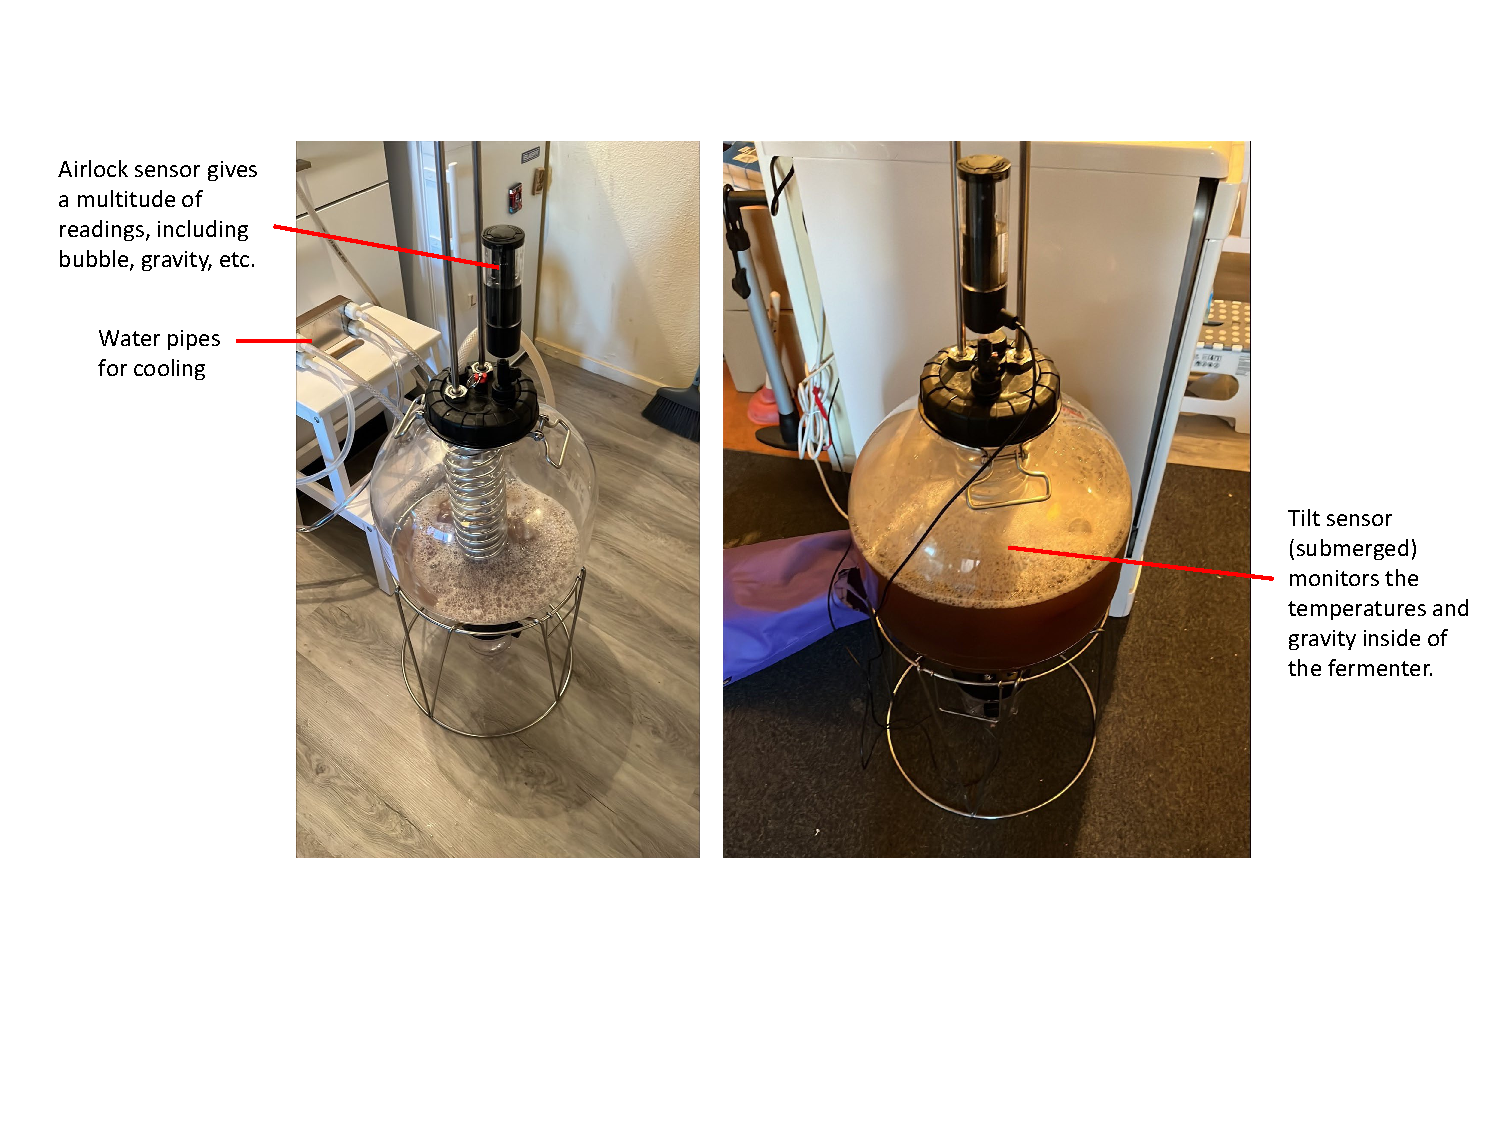
\includegraphics[scale=0.65]{figures/workbench_fermenter.pdf}
  \caption{The fermenter before (left) and after (right) being filled up with wort.}
  \label{fig:workbench_fermenter}
\end{figure}

\newpage
The other PEs that do not directly attach to the fermenter are installed in the same room, shown in Figure \ref{fig:workbench_other}. 

\begin{figure}[hbt!]
  \centering
  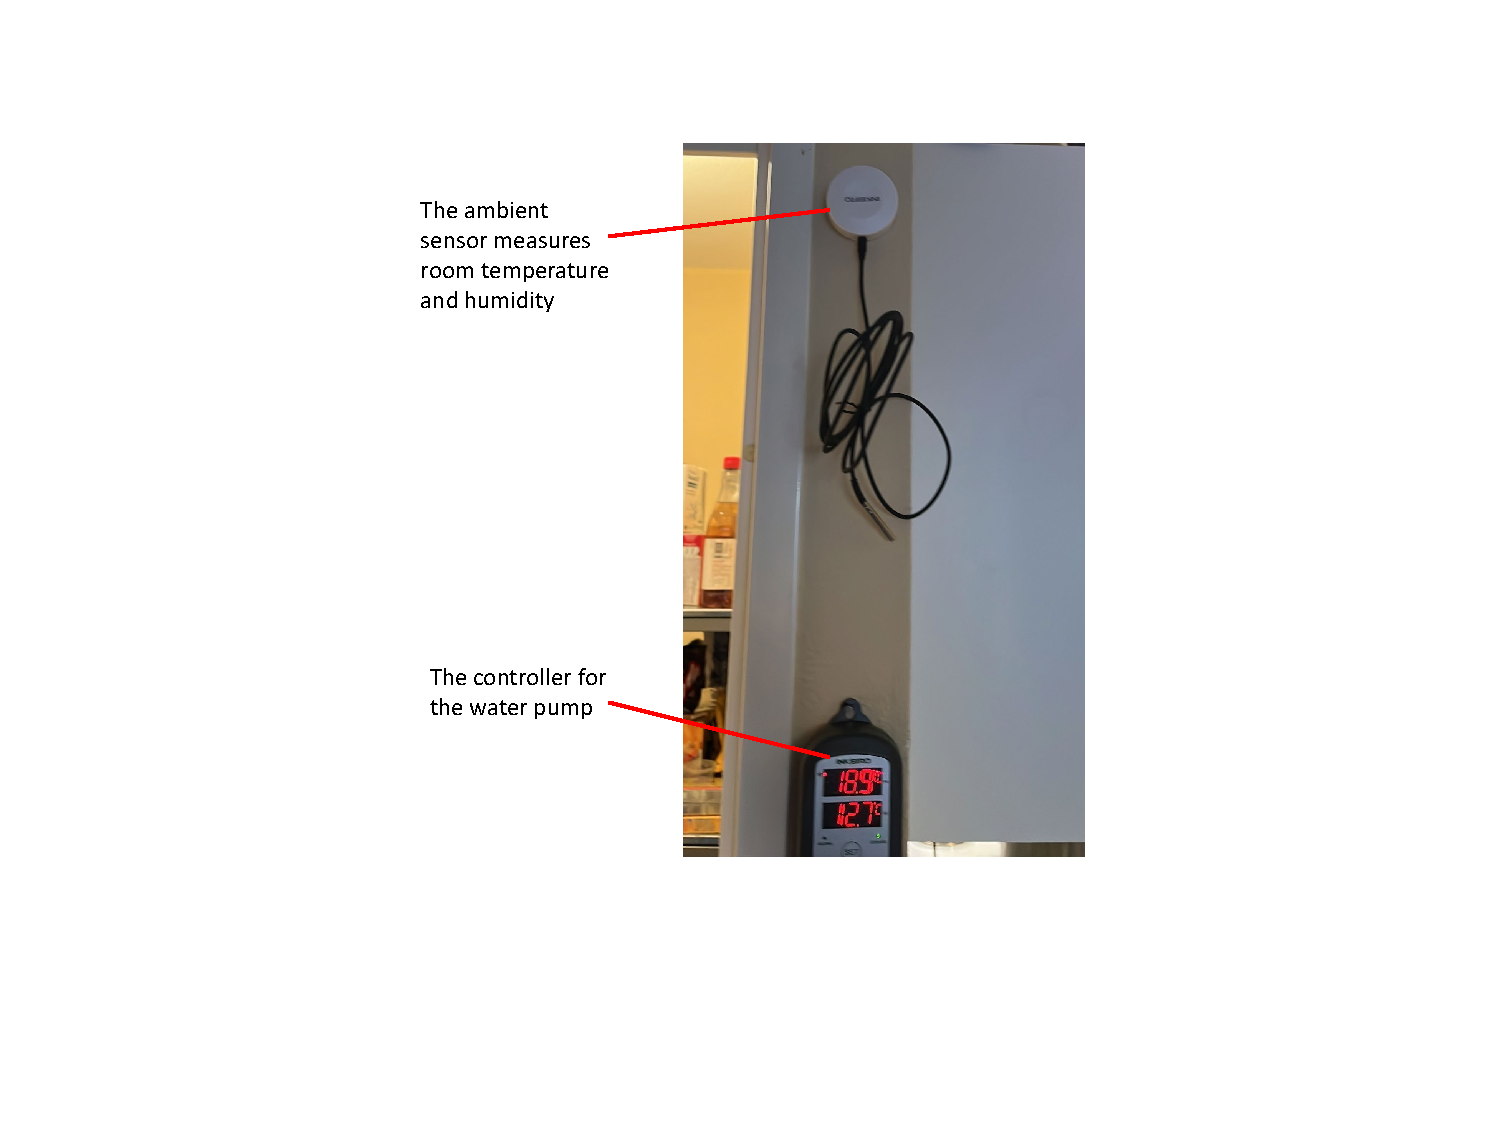
\includegraphics[scale=0.65]{figures/workbench_other.pdf}
  \caption{More devices at the workbench}
  \label{fig:workbench_other}
\end{figure}

Figure \ref{fig:workbench_map} shows the overall network topology of the workbench.

\begin{figure}[hbt!]
  \centering
  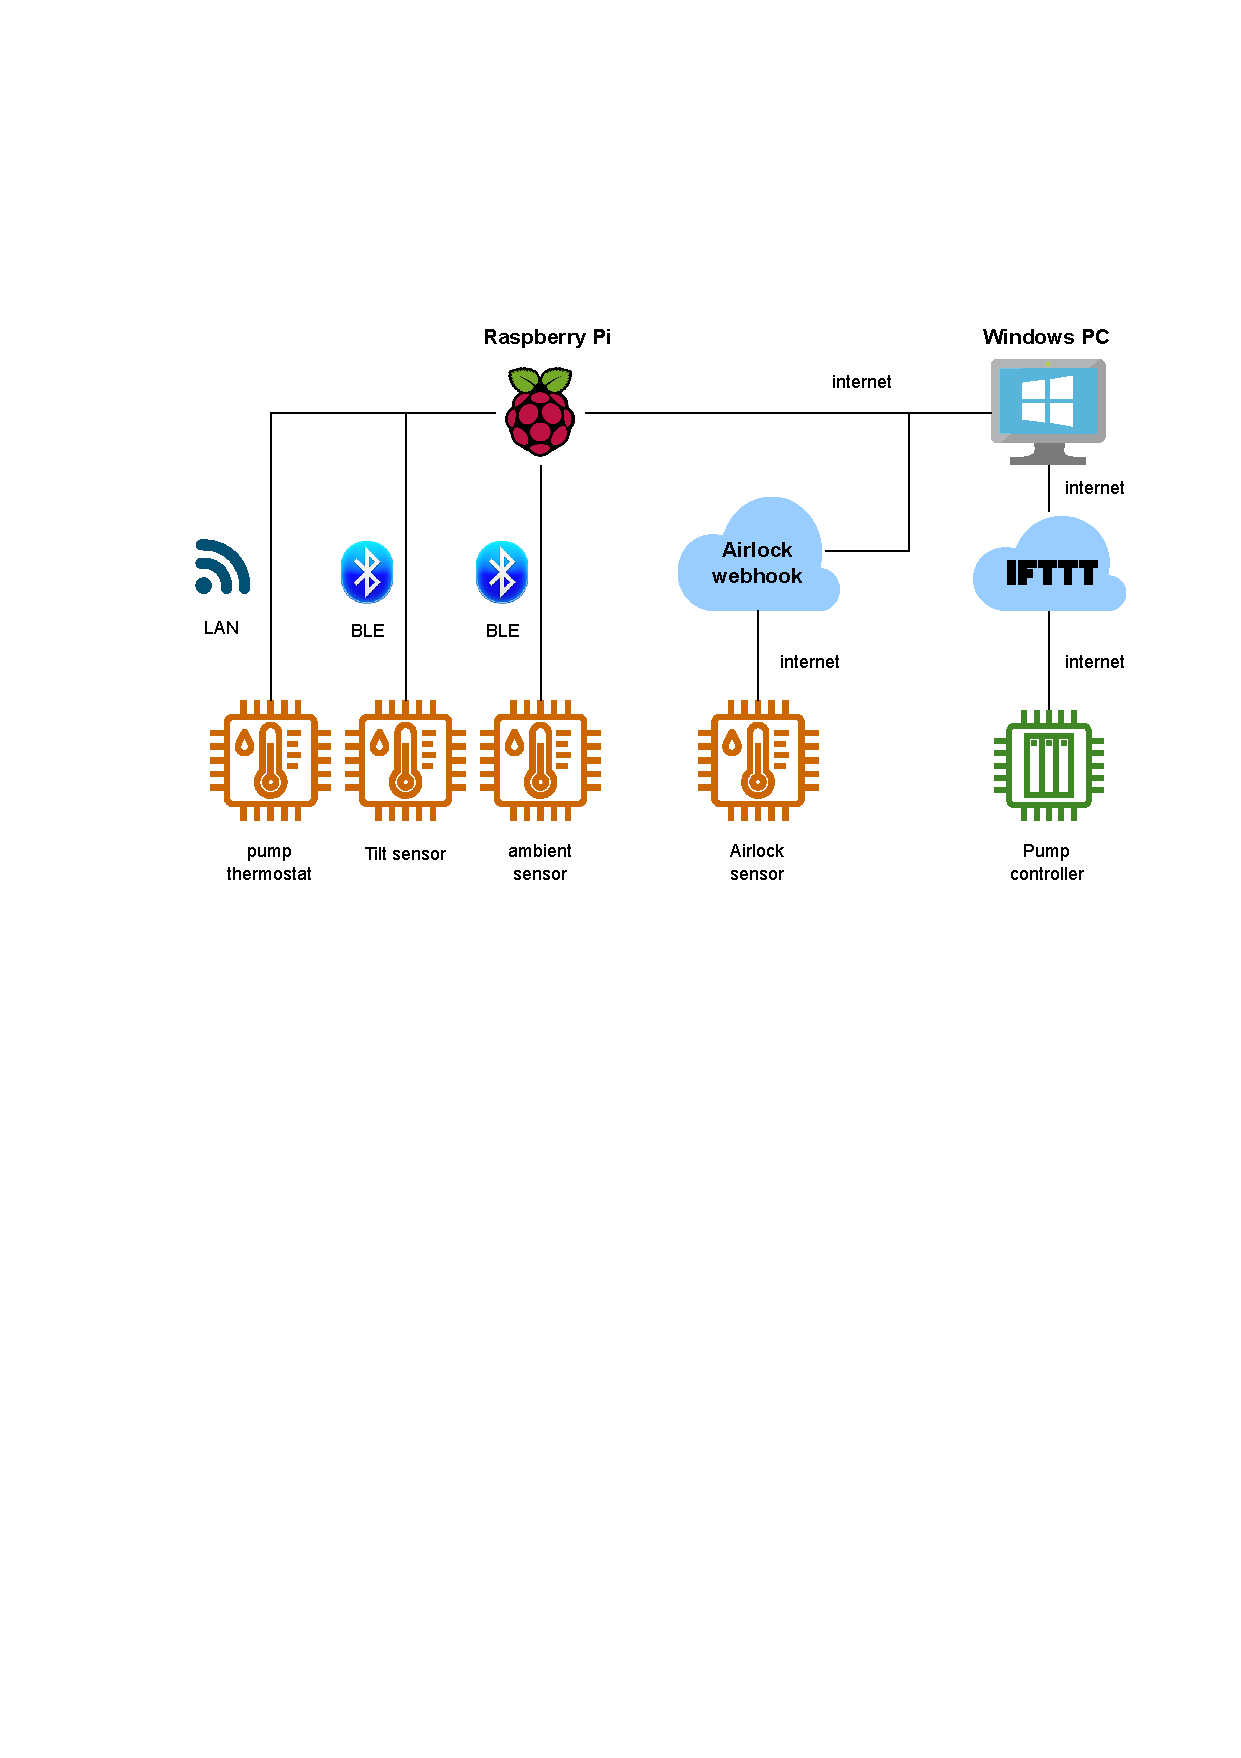
\includegraphics[scale=0.65]{figures/workbench_map.pdf}
  \caption[Network topology of the workbench]{Network topology of the workbench. Airlock sensor has an officially supported cloud server. The PC can send the control signals to the pump controller via IFTTT, which is a popular commercial service for home/smart phone automation.}
  \label{fig:workbench_map}
\end{figure}

\chapter{Kafka primer} \label{apd:kafka}
Kafka has been used extensively alongside our frameworks as a data management tool. This section will briefly introduce the main concepts of Kafka, and the advantages that make it suitable under DT contexts.

Kafka is considered an event streaming platform \cite{Kafka} that is based on the publish/subscribe design pattern (illustrated in Figure \ref{fig:kafka_example}). It supports three fundamental aspects:

\begin{figure}[hbt!]
  \centering
  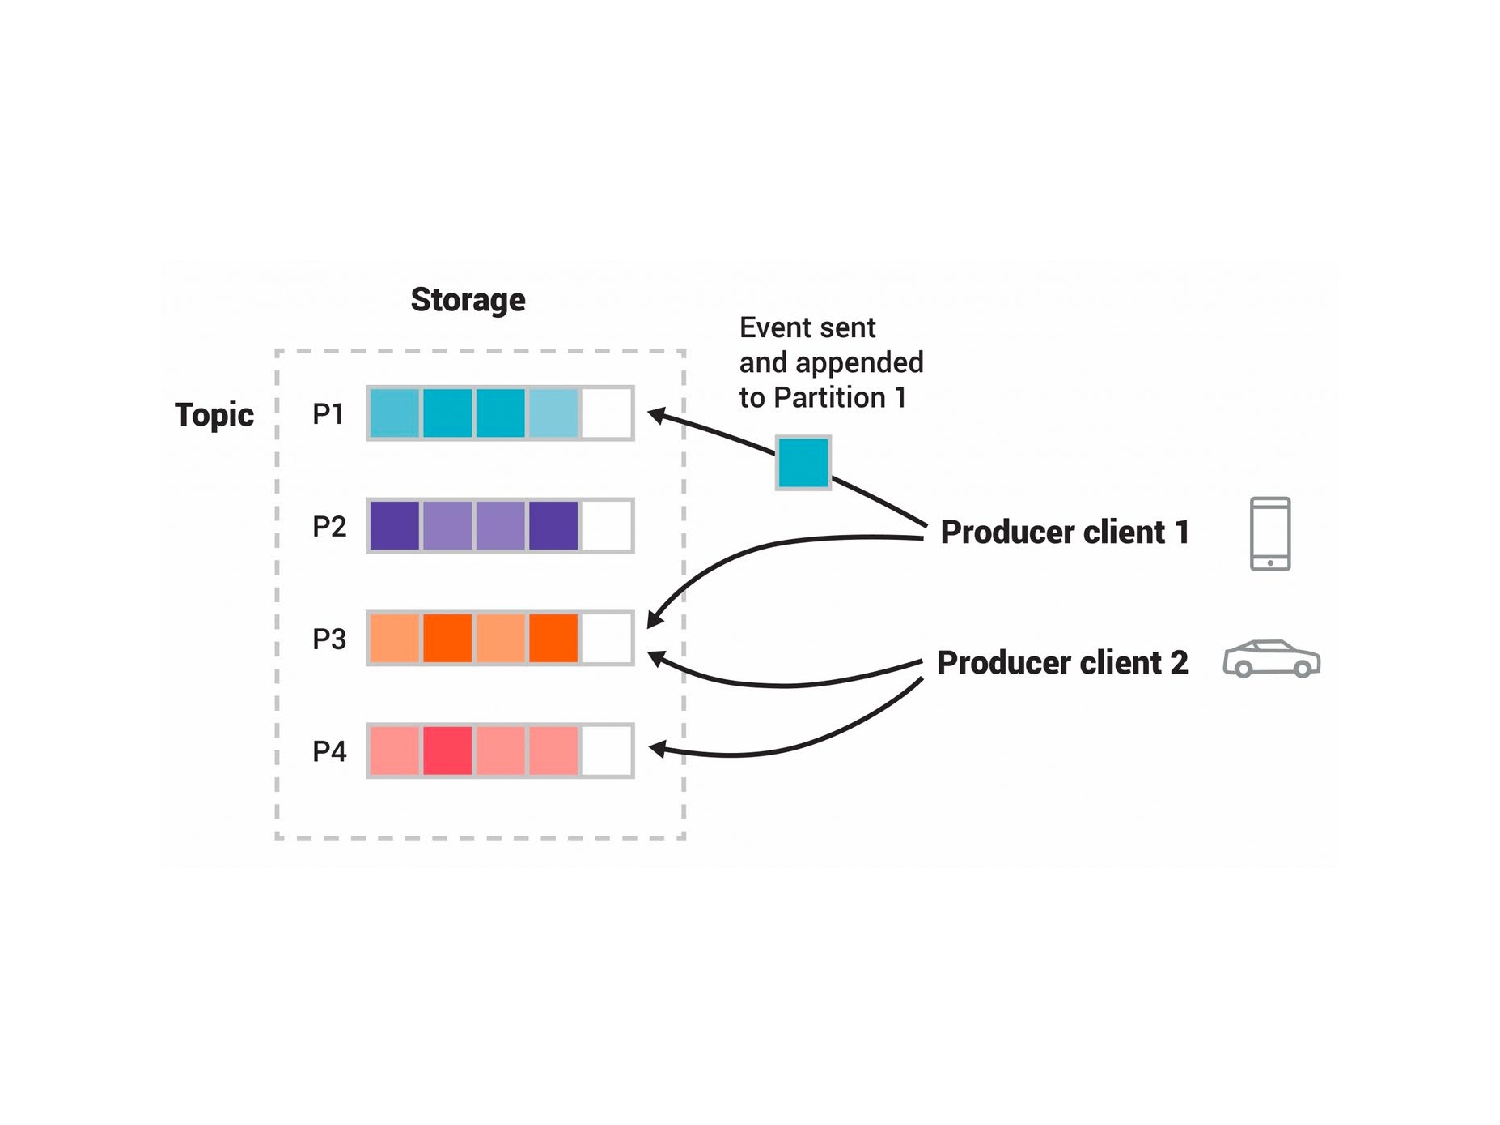
\includegraphics[scale=0.4]{figures/kafka_example.pdf}
  \caption [An example Kafka architecture] {An example Kafka architecture \cite{Kafka}}
  \label{fig:kafka_example}
\end{figure}

\begin{itemize}
\item \textbf{Publish} and \textbf{Subscribe}: the ``producer" publishes events which can be subscribed by the ``consumer". The event streams are maintained by the Kafka server such that the producer and consumer can be agnostic and decoupled to each other.
\item \textbf{Process}: referred to the enrichment and transformations of the event data. Processing can happen in real-time or in retrospect.
\item \textbf{Storage}: The event data can be stored for a duration chosen by the user.
\end{itemize} 

What makes Kafka stand out from alternative solutions of similar style (e.g., MQTT) is its emphasis on durable and persistent messages, which allows data manipulation being done either when the messages occur or retrospectively. This is important as DTs often deal with both real-time and historical data in a hybrid fashion. In Kafka the persistent storage can be accessed by ``offset tracking", a mechanism analogous to the pointer of a data structure. 

Another DT aspect Kafka manages to address is the compartmentalization of data semantics through ``topic" assignments. Conventional SQL-based approach depends on active query to data tables which sits passively in the binary objects. In contrast, Kafka turns the situation in which the data are proactively partitioned to distinct topics, while the users are ensured that different data compartments will be independent and readily accessible.  


\chapter{FMI revisit} \label{apd:fmi}
This section explains why the \texttt{FMUImporter} of Ptolemy II has failed to perform the FMUs in our case study. Our troubleshooting results indicate the root cause is due to the improper calling sequence of the FMI functions.

It begins with the FMUs used in the microbrewery DT having the property of nonlinear algebraic loop, that is, when the outputs and inputs of the model have mutual dependencies. According to the official FMI specification \cite{fmidoc}, it states that such algebraic loops may be solved in the \textit{Initialization Mode} by setting initial values to the involved inputs/outputs, which allows the solver to iteratively compute them to a convergence---when the interdependent input-output pair reaches an arbitrarily small difference. Listing \ref{lst:fmi} shows the pseudocode of what a valid calling sequence should look like.

\begin{lstlisting}[language=Python, label={lst:fmi}, caption={Resolving algebraic loop in the Initialization Mode}]
instantiate()
setupExperiment(startTime=startTime, stopTime=stopTime) 
enterInitializationMode()
setReal(inputs, values) # setting values to model variables
exitInitializationMode()
\end{lstlisting} 

However, the internal implementation of \texttt{FMUImporter} does not follow this strictly, as one can see in Figure \ref{fig:fmi_error}, in there the initialization function is terminated before setting the start values. Consequentially, the output value returns \texttt{NaN} since the FMU could not resolve the algebraic loop.

\begin{figure}[hbt!]
  \centering
  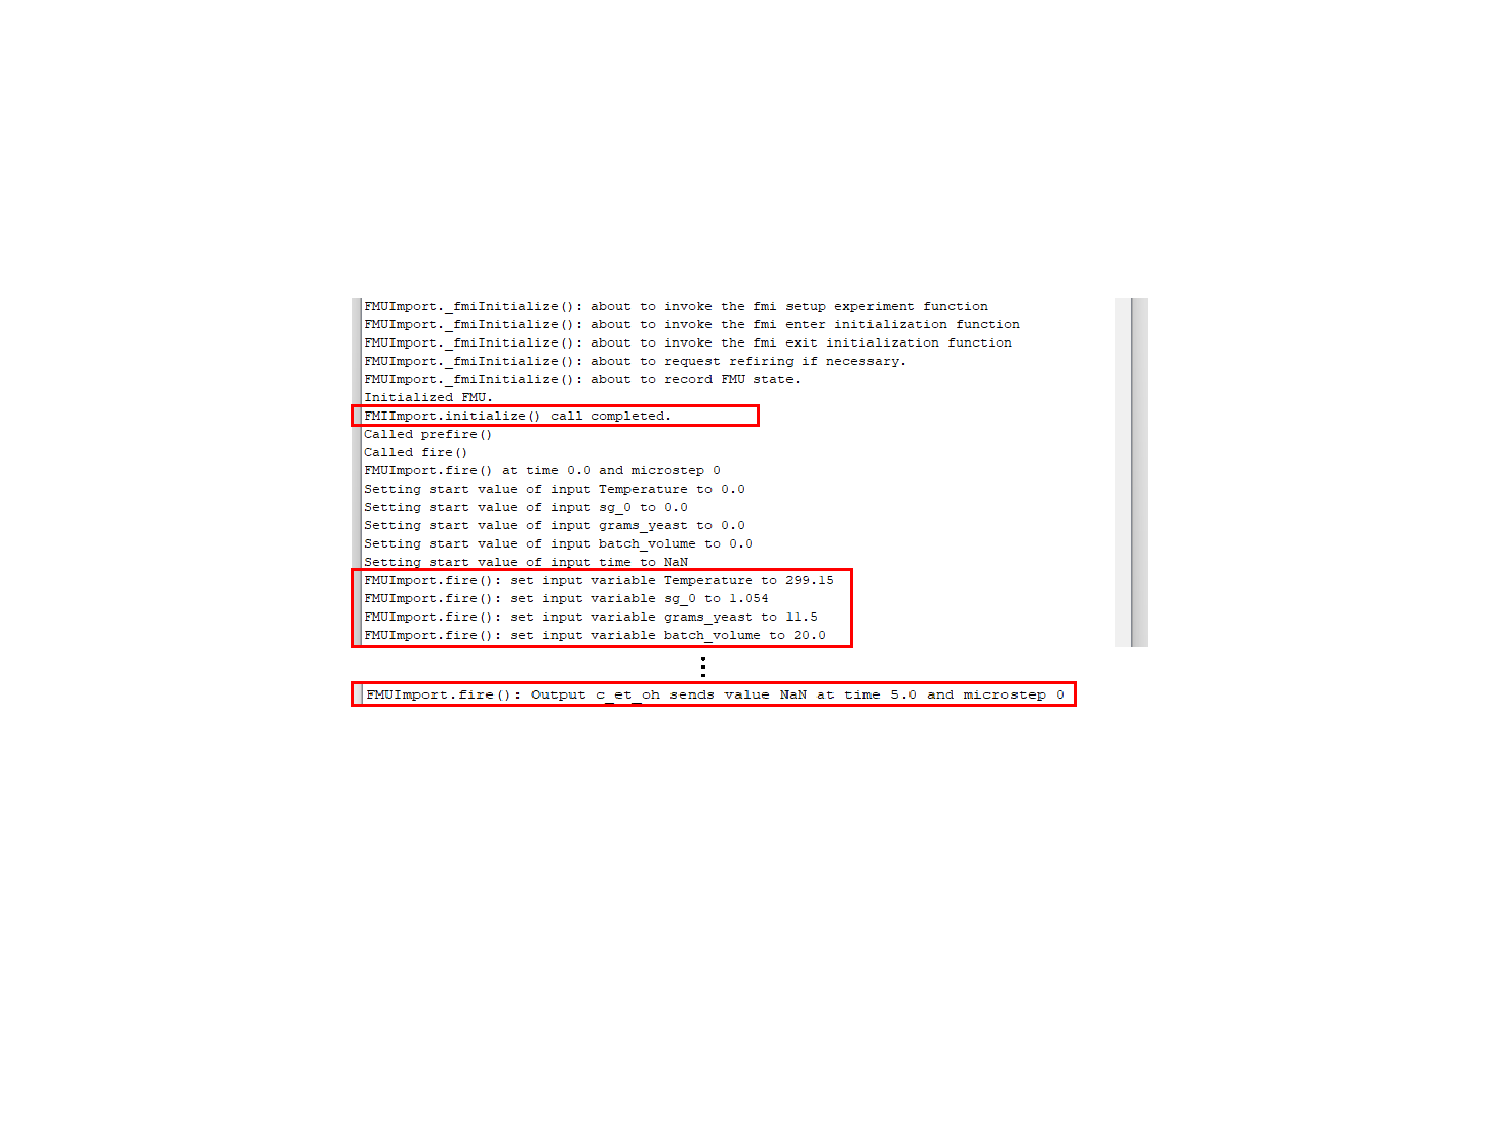
\includegraphics[scale=0.8]{figures/fmi_error.pdf}
  \caption {Incorrect function calling sequence by Ptolemy II}
  \label{fig:fmi_error}
\end{figure}

Due to this reason, along with several other limitations of Ptolemy II regarding its supports for FMI, we decide not to adopt the \texttt{FMUImporter} in the microbrewery DT implementation.

\chapter{Human-in-the-loop control scheme} \label{apd:humanloop}
This section dedicates to showcase the human-in-the-loop concept for S2---Production Control---of the microbrewery DT. For the context, a water pump is used regulate the fermentation temperature by circulating the water from a ice-cooled bucket to the fermenter and back, forming a closed water-cooling circuit. 

In the original S2, The models in VEs generate control signals that switch the power of the water pump in PEs. This operation is fully automated. Alternatively, in the human-in-the-loop version, the projection of water-cooling heat transfer is informed (via a client terminal as shown in Figure \ref{fig:hmi_client}) to the operator by the models, enabling the operator to make human judgments about replacing the ice in the bucket in order to alter the effect time of the temperature regulation. The two control schemes are illustrated Figure \ref{fig:hmi_scheme}.

\begin{figure}[hbt!]
  \centering
  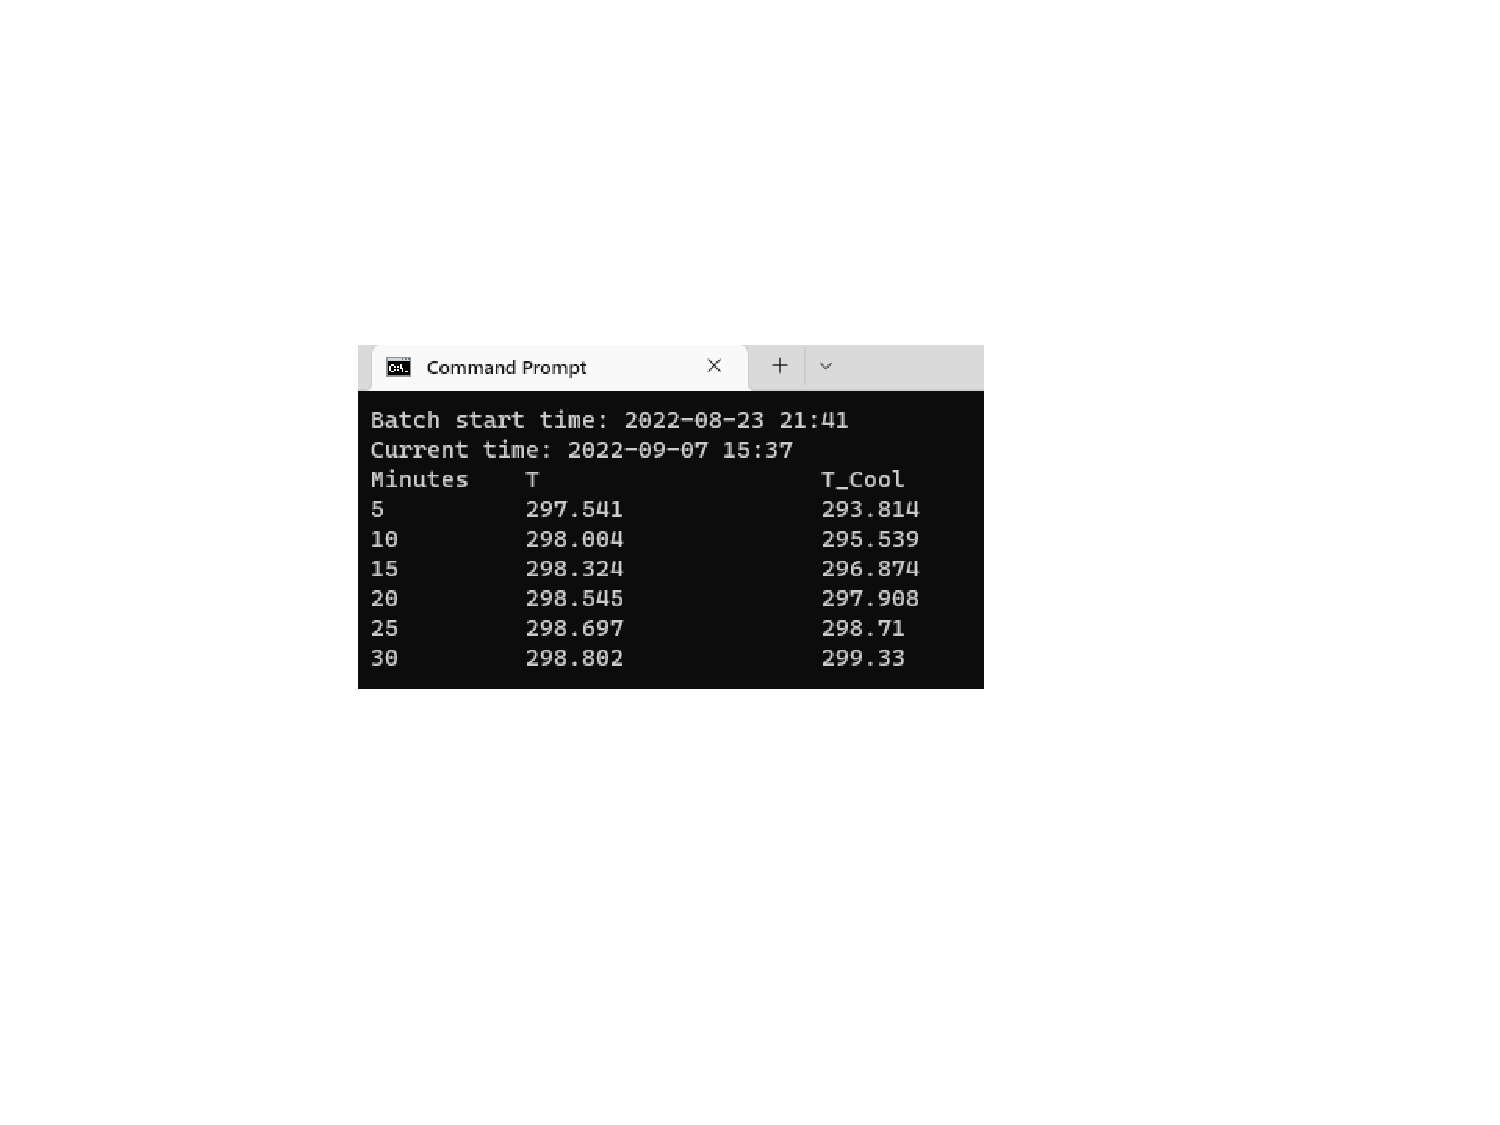
\includegraphics[scale=0.5]{figures/hmi_client.pdf}
  \caption [The client interface]{The client interface displaying a 30-minute heat predictions of the water-cooling setup}
  \label{fig:hmi_client}
\end{figure}

\begin{figure}[hbt!]
  \centering
  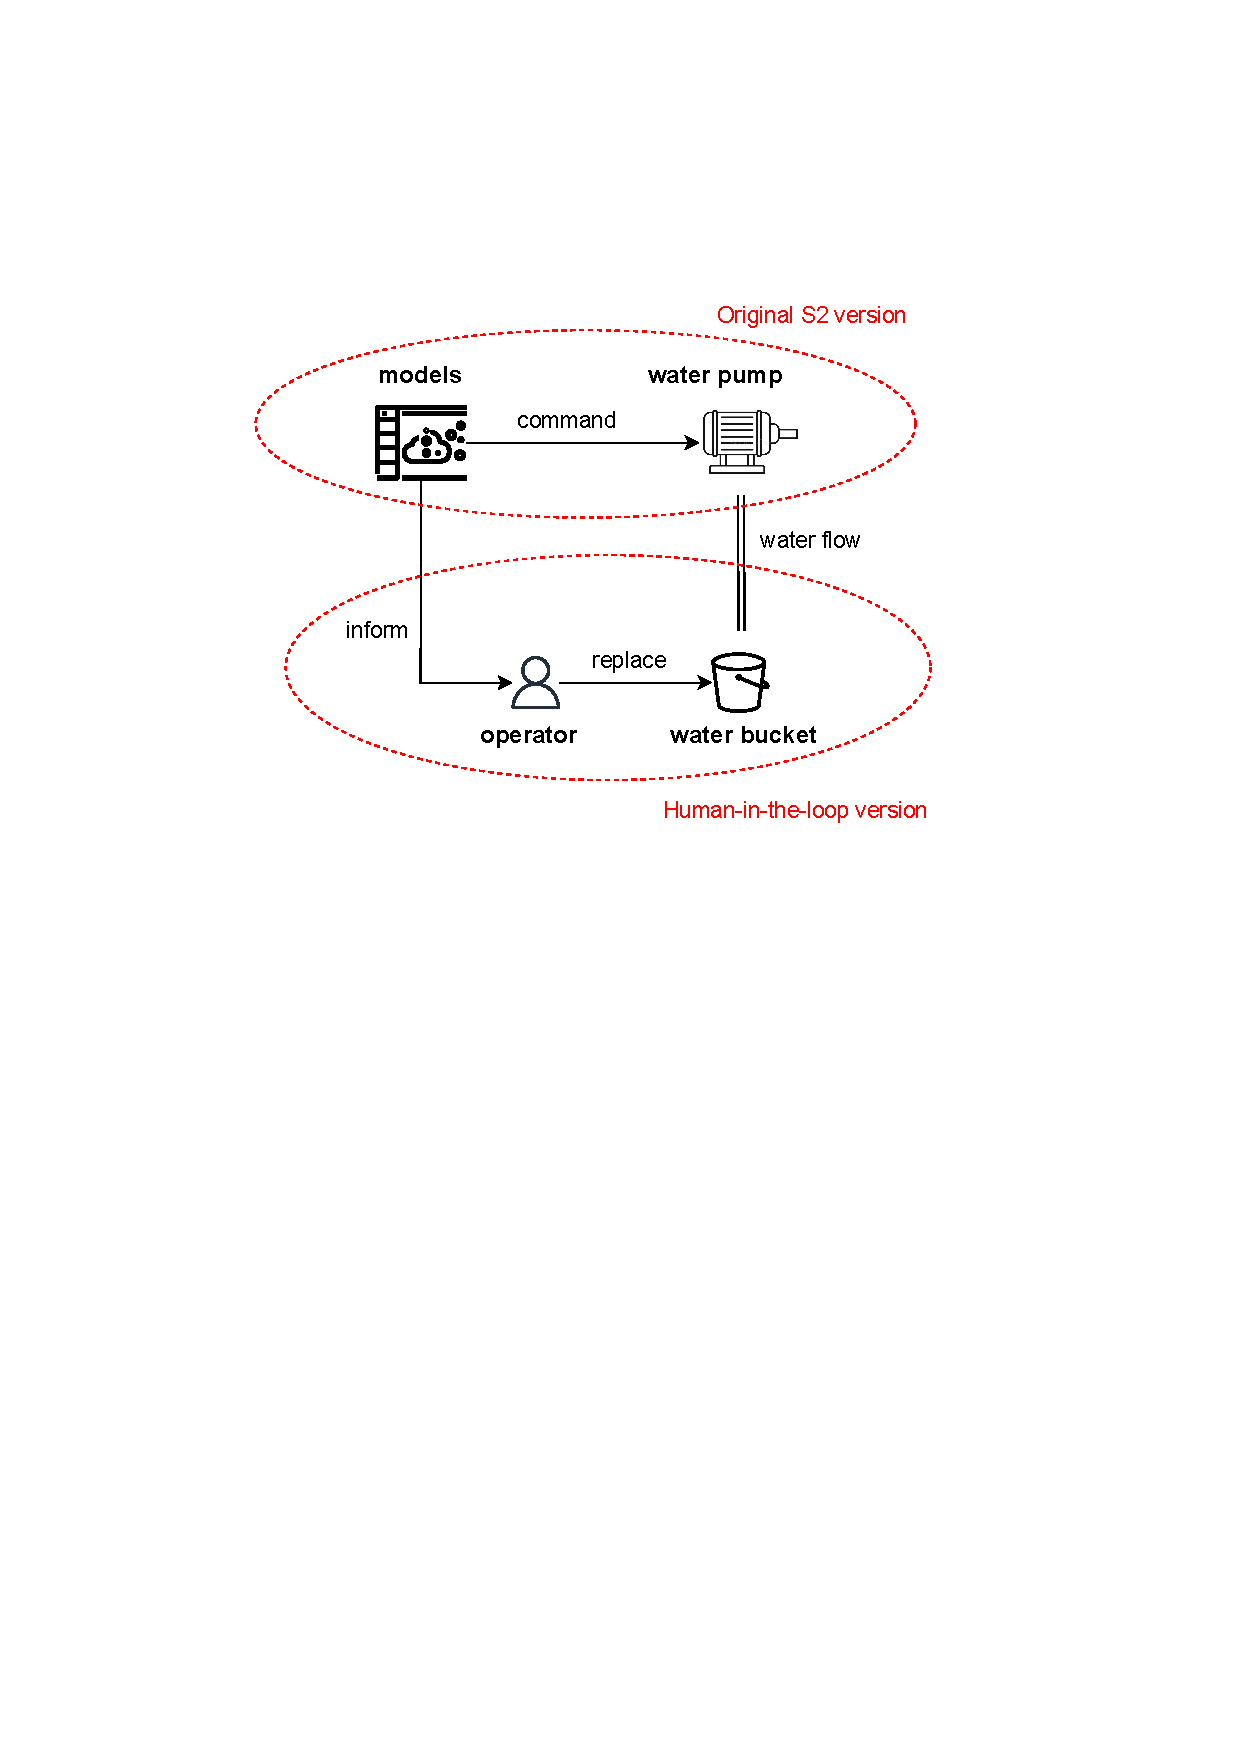
\includegraphics[scale=0.6]{figures/hmi_scheme.pdf}
  \caption {The original S2 (top) and the human-in-the-loop control scheme (bottom)}
  \label{fig:hmi_scheme}
\end{figure}

The real water circuit setup at the workbench is shown in Figure \ref{fig:workbench_bucket}.

\begin{figure}[hbt!]
  \centering
  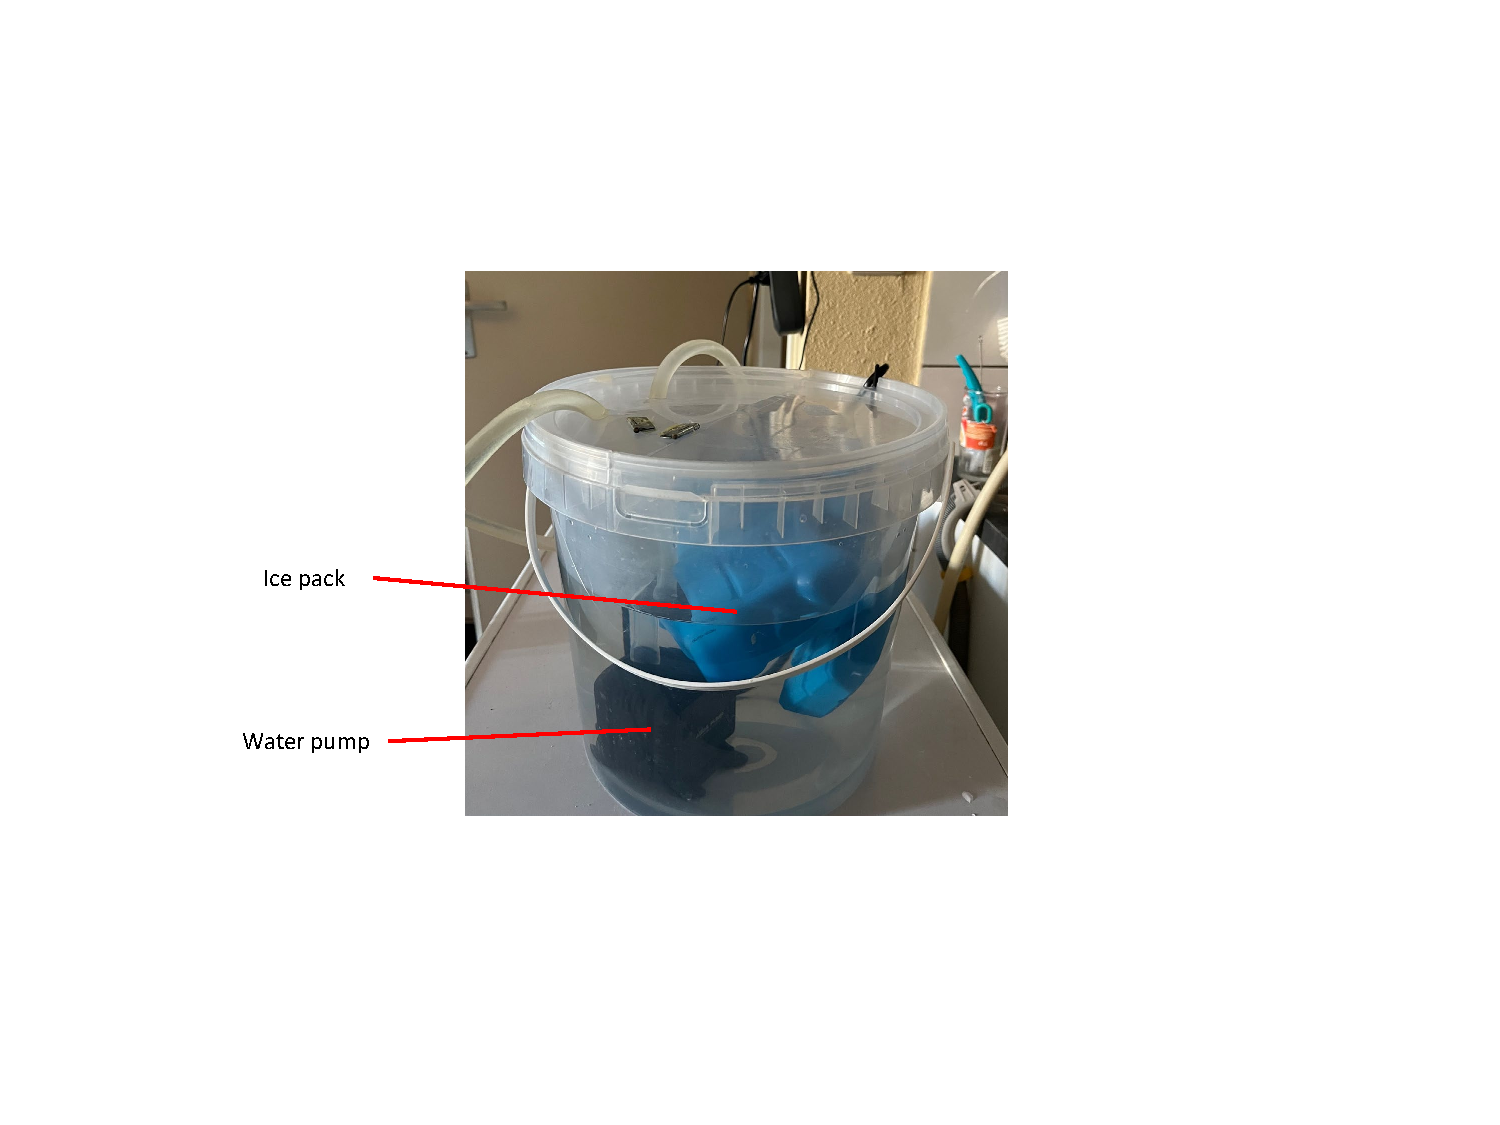
\includegraphics[scale=0.65]{figures/workbench_bucket.pdf}
  \caption{Water circuit setup}
  \label{fig:workbench_bucket}
\end{figure}

This demonstration describes a proof-of-concept for human-machine integration in a DT, although not being the primary research objective of this study, we recognize its importance for especially DTs in the bioprocessing domains.

